\msection{\Wasm}

%% For the intro
 % In 2014, Alon Zakai and colleagues proposed Emscripten \cite{emscripten}. 
% Emscripten used a strict subset of JavaScript, asm.js, to allow low-level code such as C to be compiled to JavaScript. 
% Asm.js was faster than JavaScript because it limited the language features to those that can be optimized in the LLVM pipeline. 
% Notably, Asm.js demonstrated that client-code could be improved with the right language design and standardization.
% Wasm marked the breaking point of several failed attempts of porting code but JavaScript to the web browser \cite{javaapplet,activex,silverlight}.
% Previous alternatives largely failed to gain traction, primarily due to security concerns and a lack of consensus among browser vendors.
% The announcement of \wasm\ marked the first step into the standardization of bytecode in the web environment. 

% History
The W3C publicly announced the \Wasm(Wasm) language in 2017 as the four scripting language supported in all major web browser vendors.
\wasm\ is a binary instruction format for a stack-based virtual machine and was officially consolidated by the work of Haas \etal \cite{Haas_2017} in 2017. 
It is designed to be fast, portable, self-contained and secure, and it promises to outperform JavaScript execution. 
Since 2017, the adoption of \wasm\ keeps growing. 
For example; Adobe, announced a full online version of Photoshop\footnote{\url{https://twitter.com/Adobe/status/1453034805004685313?s=20&t=Zf1N7-WmzecA0K4V8R69lw}} written in WebAssembly;  game companies moved their development from JavaScript to Wasm like is the case of a full Minecraft version\footnote{\url{https://satoshinm.github.io/NetCraft/}}. 

Moreover, WebAssembly has been evolving outside web browsers since its first announcement.
Some works demonstrated that using WebAssembly as an intermediate layer is better in terms of startup and memory usage than containerization and virtualization \cite{pMendkiServerless, 1244493Jacobsson}. 
Consequently, in 2019, the Bytecodealliance proposed WebAssembly System Interface (WASI) \cite{WASI}. 
WASI pioneered the execution of \wasm\ with a POSIX system interface protocol, making it possible to execute Wasm closer to the underlying operating system. 
Therefore, it standardizes the adoption of \wasm\ in heterogeneous platforms \cite{bryant2020webassembly}, making it suitable for standalone and backend execution scenarios \cite{9640153, wen2020wasmachine}.

% How to generate
%\msubsection{\Wasm's generation and binary format}
%\todo{Replace by Rust example}
%\todo{Annotate the Wasm code with the sections offset and length}
%\todo{Instantiate each one of the previously mentioned concepts}
%\todo{Improve some metadata, size of the code, etc}
%\todo{FIX: linerefs}

\msubsection{From source code to \Wasm}

\Wasm programs are compiled from source languages like C/C++, Rust, or Go, which means that it can benefit from the optimizations of the source language compiler.
The resulting \wasm program is like a traditional shared library, containing instruction codes, symbols, and exported functions. 
A host environment is in charge of complementing the Wasm program, such as providing external functions required for execution within the host engine. 
For instance, functions for interacting with an HTML page's DOM are imported into the Wasm binary when invoked from JavaScript code in the browser. 


In \autoref{CExample1} and \autoref{WASMExample}, we illustrate a C program and its corresponding Wasm binary. 
The C function includes heap allocation, external function usage, and a function definition featuring a loop, conditional branching, function calls, and memory accesses. 
The Wasm code in \autoref{WASMExample} displays the textual format of the generated Wasm (Wat)\footnote{The WAT text format is mostly for human readability and for low-level manual modification.}.



\begin{minipage}[hbtp]{0.9\textwidth}
    \begin{minipage}[t]{1.0\linewidth}
        \lstset{language=C,caption={Example C program which includes heap allocation, external function usage, and a function definition featuring a loop, conditional branching, function calls, and memory accesses.  },
        label=CExample1,
        breaklines=true, 
        basicstyle=\small\ttfamily,
        captionpos=b,
        frame=b,
        numbers=none,
        postbreak=\mbox{\textcolor{red}{$\hookrightarrow$}\space},
        escapeinside={(*@}{@*)}
        }
    \input{sota/code/code.c}
    \end{minipage}
\end{minipage}



\begin{minipage}[hbtp]{0.9\textwidth}
  

    \begin{minipage}[t]{1.0\linewidth}
    \lstset{
        language=WAT,
        caption={ Refer to \autoref{CExample1} for the Rust code example. This example showcases the translation from Rust to \wasm. For clarity, we have marked elements and portions of the \Wasm binary as comments.},
        style=WATStyle,
        breaklines=true, 
        %stepnumber=0,
        captionpos=b,
        frame=b,
        escapeinside={(*@}{@*)},
        numbers=none,
        postbreak=\mbox{\textcolor{red}{$\hookrightarrow$}\space},
        label=WASMExample}
    %
    \input{sota/code2/fibo.shortest.wat}
    %\end{lstlisting}
    \end{minipage}
\end{minipage}

\msubsection{\Wasm's binary format}
\label{background:wasm:binary}

The Wasm binary format is close to machine code and already optimized, being a consecutive collection of sections.
In \autoref{background:wasm:fig:section} we show the binary format of a Wasm section.
A Wasm section starts with a 1-byte section ID, followed by a 4-byte section size, and concludes with the section content, which precisely matches the size indicated earlier.
A \wasm binary contains sections of 13 types, each with a specific semantic role and placement within the module. 
Each section is optional, where an omitted section is considered empty.
In the following text, we summarize each one of the 13 types of \wasm sections, providing their name, ID, and purpose. 
In addition, some sections are annotated as comments in the Wasm code in \autoref{WASMExample}.
    
\begin{figure}[h]
    \centering
    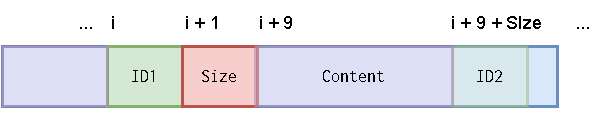
\includegraphics[width=0.5\linewidth]{figures/section.pdf}
    \caption{Memory byte representation of a \Wasm binary section, starting with a 1-byte section ID, followed by an 8-byte section size, and finally the section content.}
    \label{background:wasm:fig:section}
\end{figure}

\wrule{Custom Section (\texttt{00})}: Comprises two parts: the section name and arbitrary content. Primarily used for storing metadata, such as the compiler used to generate the binary (see lines 9 and 48 of \autoref{WASMExample}). This type of section has no order constraints with other sections and is optional. Compilers usually skip this section when consuming a \Wasm binary. 

\wrule{Type Section (\texttt{01})}: Contains the function signatures for functions declared or defined within the binary (see lines 3 to 6 in \autoref{WASMExample}). It must occur only once in a binary. It can be empty.

\wrule{Import Section (\texttt{02})}: Lists elements imported from the host, including functions, memories, globals, and tables (see line 8 in \autoref{WASMExample}). It must occur only once in a binary. It can be empty.

\wrule{Function Section (\texttt{03})}: Details functions defined within the binary. It essentially maps Type section entries to Code section entries. The text format already maps the function index to its name, as shown in lines 12 to 38 of \autoref{WASMExample}. This section must occur only once in a binary and, it can be empty. 

\wrule{Table Section (\texttt{04})}: Groups functions with identical signatures to control indirect calls. It must occur only once in a binary. It can be empty. The example code in \autoref{WASMExample} does not include a Table Section.

\wrule{Memory Section (\texttt{05})}: Specifies the number and initial size of unmanaged linear memories (see line 40 in \autoref{WASMExample}). It must occur only once in a binary. It can be empty. 

\wrule{Global Section (\texttt{06})}: Defines global variables as managed memory for use and sharing between functions in the \Wasm binary (see line 42 of \autoref{WASMExample}). It must occur only once in a binary. It can be empty.

\wrule{Export Section (\texttt{07})}: Declares elements like functions, globals, memories, and tables for host engine access (see lines 44 and 45 of \autoref{WASMExample}). It must occur only once in a binary. It can be empty.

\wrule{Start Section (\texttt{08})}:  Designates a function to be called upon binary readiness, initializing the \Wasm program state before executing any exported functions. It must occur only once in a binary. It can be empty. The example code in \autoref{WASMExample} does not include a Start Section, i.e. there is no function to call when the binary is initialized.

\wrule{Element Section (\texttt{09})}: Contains elements to initialize the binary tables. It must occur only once in a binary. It can be empty. The example code in \autoref{WASMExample} does not include an Element Section.

\wrule{Code Section (\texttt{10})}: Contains the body of functions defined in the Function section. Each entry consists of local variables used and a list of instructions (see lines 12 to 38 in \autoref{WASMExample}). It must occur only once in a binary. It can be empty.

\wrule{Data Section (\texttt{11})}: Holds data for initializing unmanaged linear memory. Each entry specifies the offset and data to be placed in memory (see line 47 in \autoref{WASMExample}). It must occur only once in a binary. It can be empty.

\wrule{Data Count Section (\texttt{12})}: Primarily used for validating the Data Section. If the segment count in the Data Section mismatches the Data Count, the binary is considered malformed. The example code in \autoref{WASMExample} does not include a Data Count Section.
It must occur only once in a binary. It can be empty.


\vspace{2mm}
Due to its organization into a contiguous array of sections, a \wasm binary can be processed efficiently. 
For example, this structure allows compilers to speed up the compilation process through parallel parsing or just by ignoring \emph{Custom Sections}.
Additionally, the use of the LEB128\toolcite{https://en.wikipedia.org/wiki/LEB128} encoding of instructions of the \emph{Code Section} further compacts the binary. 
As a result, Wasm binaries are not only fast to process but also quick to transmit over a network.

\msubsection{\Wasm's runtime structure}
\label{background:wasm:execution}


The \Wasm runtime structure is described in the WebAssembly specification by enunciating 10 key components: the Store, Module Instances,  Table Instances, Export Instances, Import Instances, the Execution Stack, Memory Instances, Global Instances, Function Instances and Locals.  
These components are particularly significant in maintaining the state of a WebAssembly program during its execution. 
In the following text, we provide a brief description of each runtime component.
Notice that, the runtime structure is an abstraction that serves to validate the execution of a \wasm binary.

\wrule{Store}: The WebAssembly store represents the global state and is a collection of instances of functions, tables, memories, and globals. Each of these instances is uniquely identified by an address, which is usually represented as an i32 integer.


\wrule{Module Instances}: A module instance is a runtime representation of a loaded and initialized WebAssembly module. 
It contains the runtime representation of all the definitions within a module, including functions, tables, memories, and globals, as well as the module's exports and imports.


\wrule{Table instances}: A table instance is a vector of function elements. 
WebAssembly tables are used to support indirect function calls.
For example, it allows modeling dynamic calls of functions (through pointers) from languages such as C/C++, for which the Wasm's compiler is in charge of populating the static table of functions.


\wrule{Export Instances}: Export instances represent the functions, tables, elements, globals or memories that are exported by a \wasm binary to the host environment. 

\wrule{Import Instances}: Import instances represent the functions, tables, elements, globals or memories that are imported into a module from the host environment. 

\wrule{The Execution Stack} holds typed values and control frames, with control frames handling block instructions, loops, and function calls.
Values inside the stack can be of the only static types allowed in Wasm 1.0, \texttt{i32} for 32 bits signed integer, \texttt{i64} for 64 bits signed integer, \texttt{f32} for 32 bits float and \texttt{f64} for 64 bits float.
Therefore, abstract types, such as classes, objects, and arrays, are not natively supported. 
Instead, during compilation, such types are transformed into primitive types and stored in the linear memory.

\wrule{Memory Instances} represent the unmanaged linear memory of a WebAssembly program, consisting of a contiguous array of bytes.
Memory instances are accessed with \texttt{i32} pointers (integer of 32 bits). 
Memory instances are usually bound in browser engines to 4Gb of size, and it is only shareable between the process that instantiates the \Wasm module and the binary itself.

\wrule{Global Instances}: A global instance is a global variable with a value and a mutability flag, indicating whether the global can be modified or is immutable.
Global variables are part of the managed data, i.e., their allocation and memory placement are managed by the host engine.
Global variables are only accessible by their declaration index, and it is not possible to dynamically address them. 


\wrule{Locals}: Locals are mutable variables that are local to a specific function instance, i.e. locals are only accessible through their index related to the executing function instance. As globals, locals are part of the managed data.

\wrule{Function Instances}: 
A function instance groups locals and a function body.
Locals are typed variables that are local to a specific function invocation as previously discussed.
The function body is a sequence of instructions that are executed when the function is called.
Each instruction either reads from the stack, writes to the stack, or modifies the control flow of the function.
Recalling the example \wasm binary previously showed, 
% Functions
the local variable declarations and typed instructions that are evaluated using the stack can be appreciated between Line 7 and Line 32 in \autoref{WASMExample}. 
Each instruction reads its operands from the stack and pushes back the result. 
In the case of \autoref{WASMExample}, the result value of the main function is the calculation of the last instruction, \texttt{i32.add}. 
As the listing also shows, instructions are annotated with a numeric type.


\begin{definition}\label{managed_unmanaged}
    Along with this dissertation, as the work of Lehmann \etal \cite{usenixWasm2020}, we refer to managed and unmanaged data to differentiate between the data that is managed by the host engine and the data that is managed by the \Wasm program respectively. 
\end{definition}


\msubsection{\Wasm's control flow}

In \Wasm, a defined function instructions are organized into blocks, with the function's starting point serving as the root block. 
Unlike traditional assembly code, control flow structures in Wasm jump between block boundaries rather than arbitrary positions within the code. 
Each block might specify the required stack state before execution and the resulting stack state after its instructions have run. 
This stack state is used to validate the binary during compilation and to ensure that the stack is in a valid state before executing the block's instructions.
Blocks in Wasm are explicit, indicating, where they start and end.
By design, each block cannot reference or execute code from outer blocks.

Control flow within a function is managed through three types of break instructions: unconditional break, conditional break, and table break. 
Importantly, each break instruction is limited to jumping to one of its enclosing blocks.
%Loops in Wasm are specialized blocks that can be restarted using a break instruction. 
Unlike standard blocks, where breaks jump to the end of the block, breaks within a loop block jump to the block's beginning, effectively restarting the loop. 
To illustrate this, \autoref{background:wasm:block} provides an example comparing a standard block and a loop block in a Wasm function.


\begin{minipage}{0.95\linewidth}
   
   \begin{minipage}{0.45\linewidth}
      \lstset{
      language=WAT,
      style=WATStyle,
      breaklines=true, 
      %stepnumber=0,
      escapeinside={(*@}{@*)},
      numbers=none,
      postbreak=\mbox{\space},
      label=BlockExample}

   \begin{lstlisting}    
block
   block
      br 1 (*@\tikzmarkMap{2}{}{8.5}{2}{2cm}@*) ; Jump instructions are annotated with the depth of the block they jump to; 
   end (*@\tikzmarkMap{7}{}{8.5}{0}{2cm}@*)
end (*@\tikzmarkMap{1}{}{8}{3}{2cm}@*)
... (*@\tikzmarkMap{9}{}{8.5}{2}{2cm}@*)
   \end{lstlisting}
   \end{minipage}\hspace{1mm}
   \begin{minipage}{0.44\linewidth}
   \lstset{
      language=WAT,
      style=WATStyle,
      breaklines=true, 
      %stepnumber=0,
      escapeinside={(*@}{@*)},
      numbers=none,
      postbreak=\mbox{\space},
      label=LoopExample}

   \begin{lstlisting}    
loop (*@\tikzmarkMap{6}{}{8.5}{2}{2cm}@*)
   ...
   br 0 (*@\tikzmarkMap{5}{}{8.5}{2}{2cm}@*) ;first-order break;
   ... 
end (*@\tikzmarkMap{3}{}{8.5}{2}{2cm}@*) ; end instructions break the block and jump to next instruction; 
... (*@\tikzmarkMap{4}{}{8.5}{-2}{2cm}@*)
   \end{lstlisting}
   \end{minipage}
   \begin{tikzpicture}[remember picture,overlay]

      %\path (2.west) edge[<-, black] (1.west);
      %\path (3.west) edge[<-,  black] (4.west);
   
      \path (1.west) edge[<-, bend right, black] (2.west);
      %\path (1.west) edge[<-, bend right, gray] (7.west);
      %\path (9.west) edge[<-, bend right, gray] (1.west);
   
      \path (4.west) edge[<-, bend right, gray] (3.west);
      \path (6.west) edge[<-, bend left, black] (5.west);
      %\path (9.east) edge[<-, bend right, black] (4.east);
      %\path (7.east) edge[<-, bend right, black] (8.east);
   
      \end{tikzpicture}
      \centering
      \hrule
      \vspace{2mm}
      \captionof{lstlisting}{Example of breaking a block and a loop in \Wasm.}
      \label{background:wasm:block}
\end{minipage}
% Example


Each break instruction includes the depth of the enclosing block as an operand. 
This depth is used to identify the target block for the break instruction. 
For example, in the left-most part of the previously discussed listing, a break instruction with a depth of 1 would jump past two enclosing blocks.


\msubsection{\Wasm's ecosystem}
\label{background:wasm:ecosystems}

%\todo{Split in two sections. Do a new section on WebAssembly analysis.}
%\todo{Other WebAssembly tools section.}

\Wasm programs are tailored for execution in host environments, most notably web browsers. 
The \Wasm ecosystem is a diverse landscape, featuring a multitude of stakeholders and a comprehensive suite of tools to meet various requirements \cite{Avenger}. 
In this section, we delineate two key categories of tools within this ecosystem: compilers and executors. 
Compilers are responsible for converting source code into \Wasm binaries, while executors handle a range of tasks including validation, analysis, optimization, machine code transpilation, and actual execution of these \Wasm binaries. 
Executors are often found in browser clients, among other platform

\wrule{Compilers} transform source code into \Wasm binaries. 
For example, LLVM has offered \Wasm as a backend option since its 7.1.0 release\toolcite{https://github.com/llvm/llvm-project/releases/tag/llvmorg-7.1.0}, supporting a diverse set of frontend languages like C/C++, Rust, Go, and AssemblyScript\footnote{A subset of the TypeScript language}.
In parallel developments, the KMM framework\toolcite{https://kotlinlang.org/docs/wasm-overview.html} has incorporated \Wasm as a compilation target, and the Javy approach\toolcite{https://github.com/bytecodealliance/javy} focuses on encapsulating JavaScript code within isolated \Wasm binaries. 
This latter is achieved by porting both the engine and the source code into a secure \Wasm environment. 
Similarly, Blazor also enables the compilation of C# code into \Wasm binaries for browser execution\footnote{\url{https://dotnet.microsoft.com/apps/aspnet/web-apps/blazor}}.

From a security standpoint, \Wasm programs are designed without a standard library and are prohibited from direct interactions with the operating system. Instead, the host environment offers a predefined set of functions that can be imported into the \Wasm program. 
It falls upon the compilers to specify which functions from the host environment will be imported by the \Wasm application.

\wrule{Browser} engines like V8\toolcite{https://chromium.googlesource.com/v8/v8.git} and SpiderMonkey\toolcite{https://spidermonkey.dev/} are at the forefront of executing \Wasm binaries in browser clients. 
These engines leverage Just-In-Time (JIT) compilers to convert \Wasm into machine code. 
This translation is typically a straightforward one-to-one mapping, given that \Wasm is already an optimized format closely aligned with machine code, as previously discussed in \autoref{background:wasm:binary}. 
For example, V8 just employs quick, rudimentary optimizations, such as constant folding and dead code removal, to guarantee fast readiness for a \wasm binary to execute.\footnote{This analysis was corroborated through discussions with the V8 development team and through empirical studies in one of our contributions\cite{CROW}} 

\wrule{Standalone engines:} \wasm has expanded beyond browser environments, largely due to the WASI\cite{WASI}. 
It standardizes the interactions between host environments and \Wasm modules through a POSIX-like interface.
\wasm compilers can generate binaries that use WASI.
Standalone engines can then execute these binaries in a variety of environments, including cloud, server, and IoT devices.
A range of standalone engines like WASM3\toolcite{https://github.com/wasm3/wasm3}, Wasmer\toolcite{https://wasmer.io/}, Wasmtime\toolcite{https://github.com/bytecodealliance/wasmtime}, WAVM\toolcite{https://github.com/WAVM/WAVM}, and Sledge\cite{Sledge} have emerged to support \Wasm and WASI. 
In a similar vein, Singh et al.\cite{WARDuino2019} introduced a virtual machine for \Wasm tailored for Arduino-based devices. 
Salim et al.\cite{trufflewasm} proposed TruffleWasm, an implementation of \Wasm hosted on Truffle and GraalVM. 
Additionally, SWAM\toolcite{https://github.com/satabin/swam} stands out as \Wasm interpreter implemented in Scala. 
Finally, WaVe\cite{wave} offers a \Wasm interpreter featuring mechanized verification of the \Wasm-WASI interaction with the underlying operating system.


\msubsection{WebAssembly binary analysis}
\todo{Check the avengers paper.}
As the WebAssembly ecosystem continues to grow, the need for robust tools to ensure its security and reliability has increased. 
To address this, a variety of tools have been developed that employ different strategies to identify vulnerabilities in \Wasm programs. 
In the following text we provide a brief overview of the most relevant tools in this space.

%% PATCH
\vspace{10mm}
\wrule{Static and dynamic analysis:} 
Tools like Wassail\cite{wassail}, SecWasm\cite{secwasm}, Wasmati\cite{wasmati}, WasmA\cite{wasma}, and Wasp\cite{Wasp} leverage techniques such as information flow control, code property graphs, control flow analysis, and concolic execution. 
Similarly, VeriWasm\cite{veriwasm} stands out as a static offline verifier specifically designed for native x86-64 binaries compiled from \Wasm. 
In the realm of dynamic analysis, tools like TaintAssembly\cite{taintassembly}, Wasabi\cite{wasabi}, and Fuzzm\cite{fuzzm} offer similar functionalities. 
Hybrid methods have also gained traction, with tools like CT-Wasm\cite{ctwasm} enabling the verifiably secure implementation of cryptographic algorithms in \Wasm. 
Stiévenart and colleagues have introduced a dynamic approach to slice \Wasm programs based on Observational-Based Slicing (ORBS)\cite{slicing, slicing2}. 
% Finally, Wafl\cite{wafl} extends AFL++ to perform coverage-based fuzzing on \Wasm binaries.


\wrule{Specialized Malware Detection:} Cryptomalwares have a wide presence in the web since the first days of \wasm.
The main reason is that mining algorithms using CPUs moved to \wasm for obvious performance reasons \cite{musch2019new}. 
In cryptomalware detection, tools like MineSweeper\cite{Minesweeper}, MinerRay\cite{MinerRay}, and MINOS\cite{MINOS} utilize static analysis through machine learning techniques to detect browser cryptomalwares. 
Conversely, tools like SEISMIC\cite{SEISMIC}, RAPID\cite{RAPID}, and OUTGuard\cite{outguard} seek the same goal with dynamic analysis techniques.
Remarkable VirusTotal\toolcite{https://www.virustotal.com}, packaging more than 60 commercial antivirus, detects cryptomalware in \wasm binaries.





%\todo{Emphasize what is missing. DO not talk about monoculture, neither diversification. Talks about runtime properties, side-channels, etc.}
%\todo{Put things into context.}
\msubsection{\Wasm's security}

As outlined, \Wasm is deterministic, well-typed, and follows a structured control flow, making it easier for compilers and engines to sandbox its execution\cite{WebAssemblySecurity}. 
Despite its robust design, the \Wasm's ecosystem is still nascent and faces security vulnerabilities, both for \Wasm consumers and with the \Wasm binaries themselves. 
For instance, Genkin et al. demonstrated that \Wasm could be exploited to exfiltrate data using cache timing-side channels\cite{Genkin2018DrivebyKC}. 
Lehmann et al. and Stiévenart and colleagues show that vulnerabilities in C/C++ source code could propagate to \Wasm binaries\cite{usenixWasm2020, DeRoover2022}.
This dissertation aims to mitigate these issues by introducing a comprehensive suite of tools designed to enhance \Wasm security through Software Diversification and to improve testing rigor within the ecosystem.

